% Taller semana 12 - FFT y sistemas de modulacion - CE 1110
%
% Compilar con pdfLaTeX. Las figuras se buscan en ../resultados/figuras/
% (las que generan los scripts de cada bloque) y en ../../resultados/figuras/
% (las de la Tarea 1, por si se reutiliza alguna).
%
% Cada bloque escribe SOLO su archivo de secciones/. D integra y uniforma.

\documentclass[11pt,letterpaper]{article}

\usepackage[utf8]{inputenc}
\usepackage[T1]{fontenc}
\IfFileExists{lmodern.sty}{\usepackage{lmodern}}{}
\IfFileExists{spanish.ldf}{\usepackage[spanish,es-nodecimaldot]{babel}}{%
  \AtBeginDocument{%
    \renewcommand{\figurename}{Figura}%
    \renewcommand{\tablename}{Cuadro}%
    \renewcommand{\refname}{Referencias}}}
\usepackage[margin=2.3cm]{geometry}
\usepackage{amsmath,amssymb}
\usepackage{graphicx}
\usepackage{booktabs}
\usepackage{float}
\usepackage{caption}
\usepackage{cite}
\usepackage[hidelinks]{hyperref}

\graphicspath{{../resultados/figuras/}{../../resultados/figuras/}}
\captionsetup{font=small,labelfont=bf}

% Marca visible de lo que falta, para que nadie entregue un TODO sin darse cuenta
\newcommand{\pendiente}[1]{\textbf{[PENDIENTE: #1]}}

\title{\vspace{-1cm}\large\bfseries Taller semana 12: FFT y sistemas de modulación\\[4pt]
\normalsize\mdseries Avance del Proyecto Grupal 1}

\author{%
\normalsize Santiago Brenes Torres \quad\textbullet\quad Kevin Antonio Carranza Blanco\\[2pt]
\normalsize Luis David Delgado Jiménez \quad\textbullet\quad Gretchell Roxana Ochoa Quintero\\[3pt]
\small Escuela de Ingeniería en Computadores, Instituto Tecnológico de Costa Rica\\[-1pt]
\small CE\,1110 --- Análisis de Señales Mixtas}

\date{\small 30 de octubre de 2026}

\begin{document}
\maketitle

% Introduccion - la escribe D al integrar (media pagina como maximo)

\section{Introducción}

El taller pide tres cosas sobre el mismo sistema del Proyecto 1: prototipar en
alto nivel las frecuencias con las que se va a trabajar, generar en el
microcontrolador el emisor de esas señales, y definir con diagramas cómo se va a
validar lo que el receptor recibe. No es un ejercicio aparte: lo que aquí se
decide es el banco de pruebas con el que después se va a medir el sistema
distribuido de reducción de ruido.

El montaje tiene dos placas. Una Raspberry Pi Pico hace de emisor y sintetiza por
PWM, con un filtro RC a la salida, tres modos de señal; una Pico W hace de nodo 1
y las captura por su ADC, las transforma por bloques y reporta lo que midió. Los
tres modos no se eligieron al azar: el modo 1 es un tono de 440\,Hz, el modo 2 el
multitono de 440, 880 y 1320\,Hz, y el modo 3 ese multitono más una interferencia
de 3500\,Hz con la misma relación señal a ruido del \texttt{caso\_1} de la Tarea 1.
Así cada modo corresponde a una prueba que el proyecto ya tenía definida, y los
resultados del taller se pueden comparar directamente con los que se midieron en
simulación.

Ningún número de este documento está escrito a mano en el código. Los parámetros
que vienen de la Tarea 1 --- frecuencia de muestreo de 16\,kHz, bloques de 1024
muestras, ventana Hann y 50\,\% de solapamiento --- se leen de
\texttt{metadatos/configu\-raciones.json}, y los que agrega el taller --- los modos
del emisor, los datos del receptor y los márgenes de validación --- de
\texttt{taller\_semana12/parametros.json}. Si en la defensa se cambia un
parámetro, se cambia en el JSON y todo lo demás lo sigue.

El documento está organizado por bloques, en el orden en que se recorre la señal.
La sección \ref{sec:senales} justifica la frecuencia de muestreo y el tamaño de
bloque y define la señal exacta de cada modo, que es la referencia que usan todos
los demás. La sección \ref{sec:sistema} arma el sistema completo en alto nivel. La
sección \ref{sec:emisor} lo baja al microcontrolador. La sección
\ref{sec:validacion} define la estrategia de validación en el receptor con sus
cuatro diagramas y los criterios de aceptación. La sección \ref{sec:discusion}
cierra con lo que funcionó, las limitaciones y lo que cambia para el proyecto.

% Bloque A - Senales y frecuencias - rama taller-senales
% Figuras: a_*.png que genera a_senales/prototipo_frecuencias.py
% Cifras: salida de ese script y resultados/a_dft_vs_fft.csv

\section{Frecuencias de trabajo}
\label{sec:senales}

\subsection{Frecuencia de muestreo y tamaño de bloque}

Se conservan los parámetros de la Tarea~1: $f_s = 16$\,kHz y bloques de
$N = 1024$ muestras con ventana Hann y 50\,\% de solapamiento. La componente
más alta que genera el emisor es la interferencia de 3500\,Hz, menos de la
mitad de la frecuencia de Nyquist ($f_s/2 = 8$\,kHz), así que ninguna se pliega
y queda margen para que el filtro de reconstrucción del emisor y el
antialiasing del receptor tengan una banda de transición amplia. El script
verifica esta condición con cada frecuencia del archivo de parámetros y se
detiene si alguna la viola.

Con $N = 1024$ la resolución es $\Delta f = f_s/N = 15{,}625$\,Hz y cada bloque
dura $N/f_s = 64$\,ms. Los tonos útiles están separados 440\,Hz, unos
28~bins, de modo que se distinguen con holgura aun con el lóbulo principal de
la ventana Hann, que ocupa 4~bins. Que $N$ sea potencia de dos permite usar la
FFT radix-2 de la Tarea~1 sin rellenar con ceros.

Los dos microcontroladores admiten esta $f_s$. El ADC de la Pico~W (RP2040,
12~bits) muestrea hasta 500\,kS/s, así que 16\,kS/s usa una fracción pequeña de
su capacidad. En el emisor, la portadora PWM de 8~bits (tope 255) oscila a
$125\,\text{MHz}/256 \approx 488$\,kHz, unas 30 veces la frecuencia de muestreo
y unas 140 veces la componente más alta, lo que facilita separarla con un
filtro RC. El reloj de muestreo sale de otra rebanada PWM con divisor 2,5:
$125\,\text{MHz}/(2{,}5 \cdot 16\,\text{kHz}) = 3125$ y
$133\,\text{MHz}/(2{,}5 \cdot 16\,\text{kHz}) = 3325$ son enteros, así que el
tope $3125-1$ (o $3325-1$) da 16\,kHz exactos con cualquiera de los dos relojes.

\subsection{Modos del emisor}

El cuadro~\ref{tab:modos} resume los tres modos. Las amplitudes relativas son
las de la Tarea~1. La salida se escala por $0{,}8/\sum_i A_i$, que es lo mismo
que calcula el emisor: si todas las componentes coincidieran en su pico la suma
valdría exactamente 0,8 del rango del PWM, y así nunca satura. Como en el
emisor todos los acumuladores de fase arrancan en cero, la referencia de Python
también usa fase cero en todas las componentes. Esta referencia es
\texttt{senal\_del\_modo()} y la usan los bloques B, C y D.

\begin{table}[H]
\centering\small
\caption{Modos del emisor. $k = f/\Delta f$ es la posición en bins con
$N = 1024$. Amplitud de salida = amplitud relativa $\times$ escala.}
\label{tab:modos}
\begin{tabular}{clrrrrc}
\toprule
Modo & Uso & $f$ (Hz) & Amp.\ relativa & Amp.\ de salida & $k$ & ¿Bin exacto? \\
\midrule
1 & prueba P1        & 440  & 1,00   & 0,800 & 28,16  & no \\
\midrule
2 & prueba P2        & 440  & 1,00   & 0,432 & 28,16  & no \\
  &                  & 880  & 0,55   & 0,238 & 56,32  & no \\
  &                  & 1320 & 0,30   & 0,130 & 84,48  & no \\
\midrule
3 & caso\_1          & 440  & 1,00   & 0,287 & 28,16  & no \\
  &                  & 880  & 0,55   & 0,158 & 56,32  & no \\
  &                  & 1320 & 0,30   & 0,086 & 84,48  & no \\
  & (interferencia)  & 3500 & 0,9373 & 0,269 & 224,00 & sí \\
\bottomrule
\end{tabular}
\end{table}

Ningún tono útil cae en un bin exacto. Un bloque de 1024 muestras no contiene un
número entero de periodos de estas componentes, y al repetirlo la FFT ve un
salto en los bordes que reparte la energía en muchos bins (fuga espectral). Con
ventana rectangular los lóbulos laterales empiezan en $-13$\,dB y caen
despacio, así que la fuga de 440\,Hz taparía los tonos más débiles. La ventana
Hann lleva la señal a cero en los bordes: su primer lóbulo lateral está en
$-31$\,dB y los siguientes caen 18\,dB por octava. A cambio, el lóbulo principal
se ensancha a 4~bins y el pico puede perder hasta 1,4\,dB cuando el tono cae
entre dos bins. Con la separación de 28~bins entre tonos, ese costo no afecta.
La interferencia de 3500\,Hz cae exactamente en el bin 224.

\paragraph{SNR del modo 3.} Las componentes tienen frecuencias distintas y son
ortogonales, así que la potencia de cada una es $A^2/2$ y las potencias se
suman. Los tres tonos útiles suman
$P_u = (1^2 + 0{,}55^2 + 0{,}3^2)/2 = 0{,}69625$ y la interferencia
$P_r = 0{,}9373^2/2 = 0{,}43927$, de donde
$\text{SNR} = 10\log_{10}(P_u/P_r) = 2{,}0004$\,dB, la misma que el
\texttt{caso\_1} (2\,dB). La amplitud exacta sería 0,937341; el redondeo a cuatro
decimales mueve la SNR menos de 0,001\,dB. La escala común del emisor multiplica
todas las componentes por el mismo factor y no cambia la SNR.

\subsection{Espectros esperados}

La figura~\ref{fig:espectros} muestra el espectro de un bloque de cada modo
antes y después de cuantizar a los 8~bits del PWM. Las magnitudes están
corregidas por la ganancia de la ventana, así que un tono de amplitud $A$ sale
en $20\log_{10}A$ cuando cae en un bin exacto. El tono de 3500\,Hz (bin 224)
sale en $-11{,}40$\,dB, igual a $20\log_{10}0{,}269$. Los tonos que caen entre
bins salen un poco más bajos por la pérdida de la Hann: 440\,Hz (bin 28,16)
pierde 0,14\,dB y 1320\,Hz (bin 84,48, casi a medio bin) pierde 1,3\,dB.

Con un paso $\Delta = 2/2^8$ y error uniforme, la potencia del ruido de
cuantización es $\Delta^2/12$. Frente a un seno de amplitud completa eso da una
SNR de $6{,}02\cdot 8 + 1{,}76 = 49{,}9$\,dB. En el espectro ese ruido se
reparte entre los bins: con $N = 1024$ y el ancho de banda equivalente de la
ventana Hann (1,5~bins), cada bin recibe $10\log_{10}(N/(2\cdot 1{,}5)) =
25{,}3$\,dB menos, y el piso por bin queda en $-75{,}3$\,dB. Las curvas ideal y
cuantizada coinciden en los picos; lo que cambia es el fondo lejos de los tonos,
que sube de menos de $-100$\,dB a cerca del piso teórico.

El error de cuantización no es exactamente ruido blanco. La señal es periódica
(440, 880 y 1320\,Hz se repiten juntas cada 400 muestras) y el error también,
así que se concentra en líneas en lugar de repartirse parejo. El caso extremo es
el modo~1, con un solo tono: la mediana del fondo queda en $-87$\,dB, pero
algunas líneas llegan a $-61$\,dB. Aun así quedan casi 60\,dB por debajo del
tono, y en los modos 2 y 3 ninguna línea pasa de $-63$\,dB. Un ADC ideal de
12~bits tendría un piso 24\,dB más bajo, así que en principio domina la
cuantización del emisor. El ADC real del RP2040 tiene menos bits efectivos que
12, y conviene medirlo en el receptor.

Esta referencia no modela el truncamiento de fase del DDS, que indexa una tabla
de 256 muestras con los 8~bits altos del acumulador. Ese truncamiento agrega
espurios propios que el bloque~C debe medir en la salida real
(sección~\ref{sec:emisor}). Para que la comparación muestra a muestra tenga
sentido, el emisor debe pasar de $[-1,1)$ al nivel PWM igual que
\texttt{cuantizar()}: $\text{nivel} = \text{round}(128\,x) + 128$, limitado
a 0--255.

\begin{figure}[H]
\centering
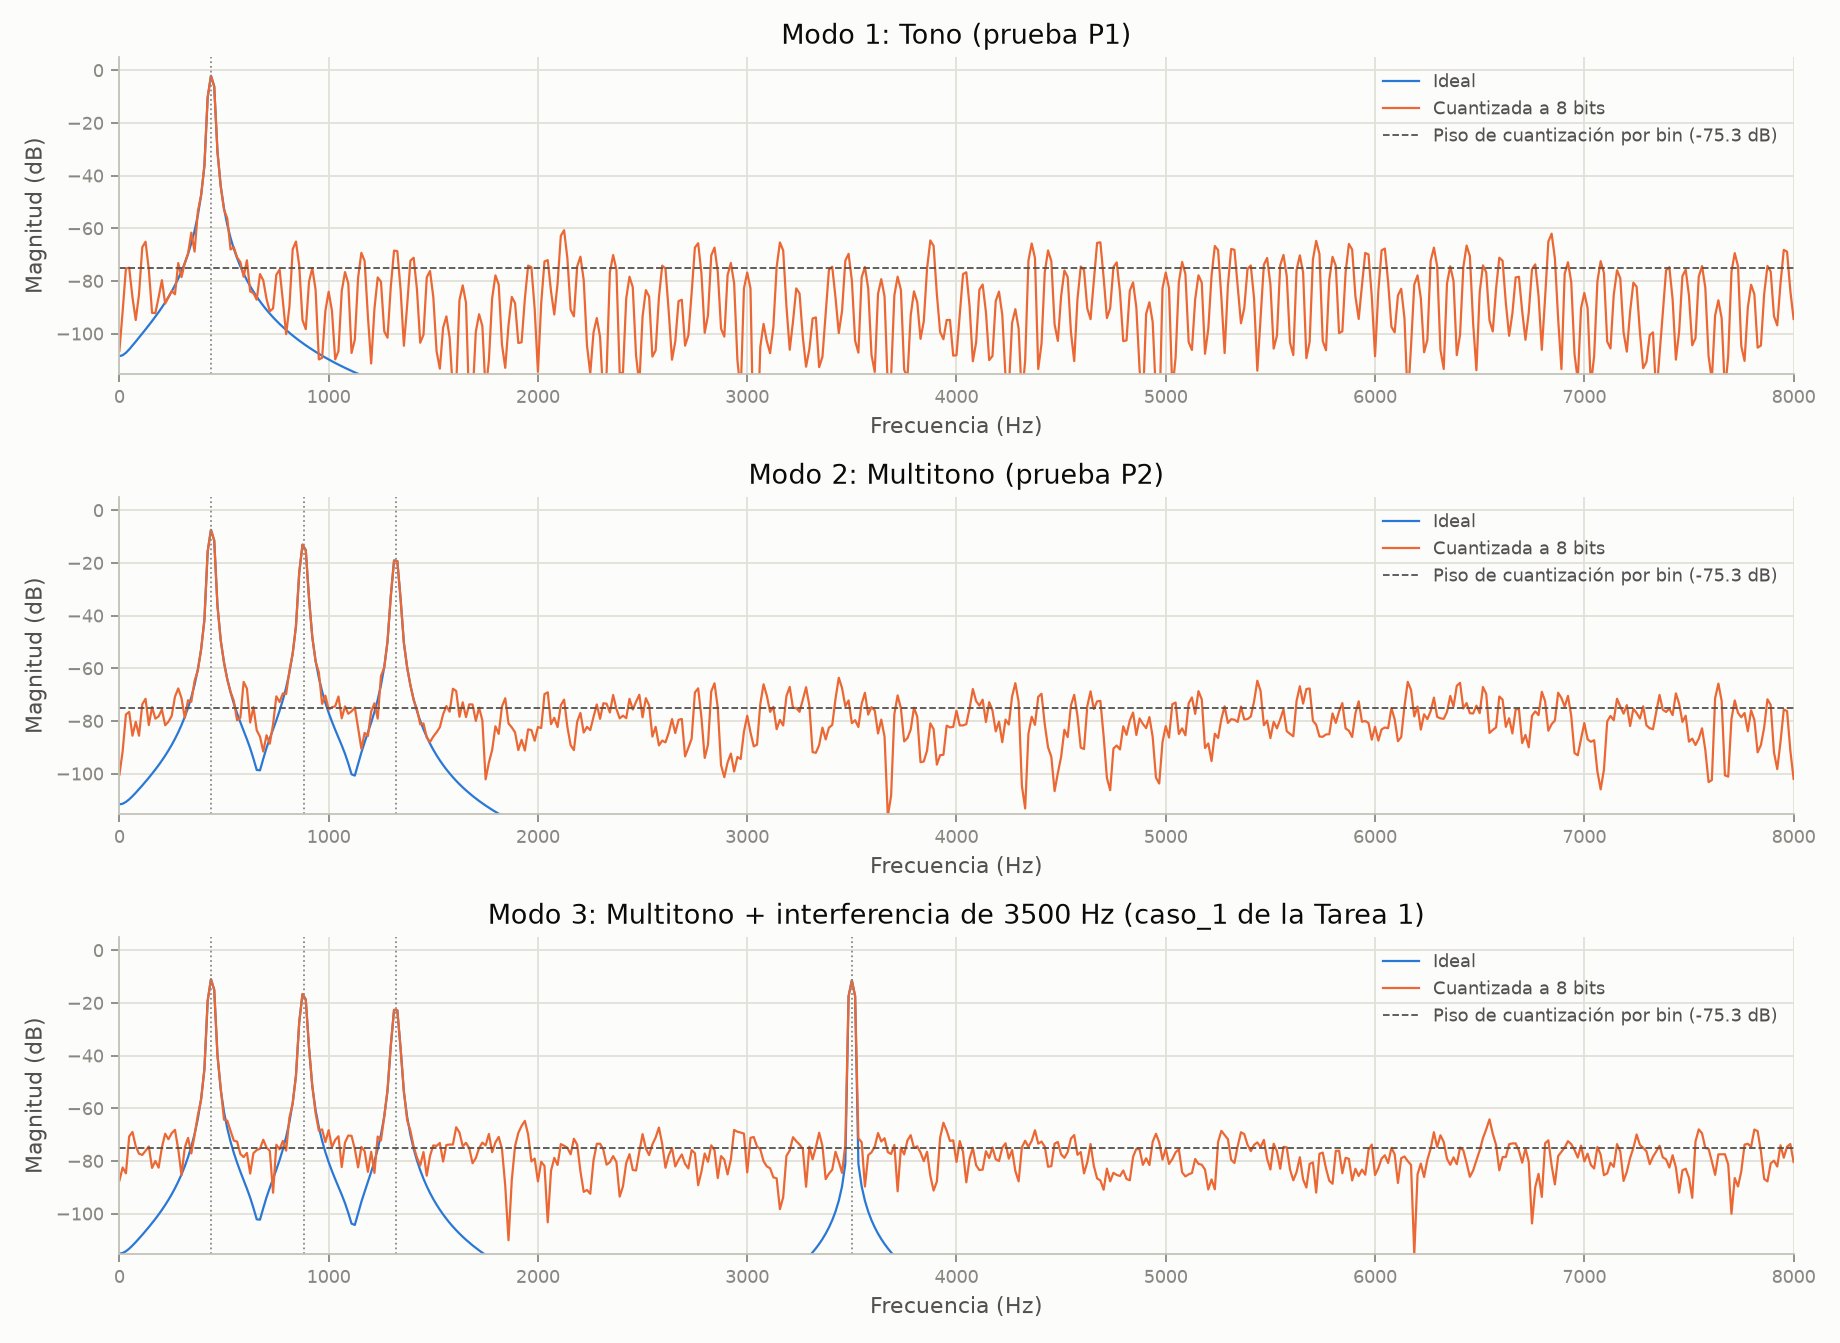
\includegraphics[width=\linewidth]{a_espectros_modos.png}
\caption{Espectro de un bloque ($N = 1024$, ventana Hann) de cada modo del
emisor, ideal y cuantizado a 8~bits. Las líneas punteadas verticales marcan las
frecuencias esperadas y la horizontal, el piso teórico de cuantización por bin.}
\label{fig:espectros}
\end{figure}

\subsection{DFT frente a FFT}

El cuadro~\ref{tab:dft_fft} compara la DFT por definición (\texttt{dft()},
dos lazos explícitos) y la FFT radix-2 iterativa (\texttt{fft()}) de
\texttt{src/dft\_fft.py}, con un bloque del modo~3 de $N = 1024$ muestras. El
tiempo es el promedio de 3 corridas de la DFT y de 50 de la FFT, en Python y en
la computadora de desarrollo. Los valores absolutos dependen de la máquina; la
razón entre ellos depende mucho menos.

\begin{table}[H]
\centering\small
\caption{DFT por definición frente a FFT radix-2 con $N = 1024$.}
\label{tab:dft_fft}
\begin{tabular}{lrr}
\toprule
 & DFT & FFT \\
\midrule
Multiplicaciones complejas & $N^2 = 1\,048\,576$ & $\tfrac{N}{2}\log_2 N = 5120$ \\
Tiempo promedio            & 858\,ms             & 4,06\,ms \\
\midrule
Razón medida / teórica     & \multicolumn{2}{c}{212 / 205} \\
Error máximo $|X_\text{DFT} - X_\text{FFT}|$ & \multicolumn{2}{c}{$4{,}0\times10^{-11}$} \\
\bottomrule
\end{tabular}
\end{table}

La aceleración medida (212 veces) coincide con la teórica
($2N/\log_2 N = 205$). No es idéntica porque el tiempo no es solo de
multiplicaciones: la DFT también evalúa una exponencial compleja por término, y
la FFT resuelve cada etapa con operaciones vectoriales de NumPy. El error máximo es $4\times 10^{-11}$ cuando el bin más
grande vale 141, un error relativo cercano a $3\times10^{-13}$, que es
redondeo de punto flotante. Las dos dan el mismo resultado. En el
microcontrolador la diferencia decide si el sistema es viable: cada bloque de
64\,ms exige 5120 multiplicaciones complejas con la FFT frente a más de un
millón con la DFT.

% Bloque B - Sistema completo en alto nivel - rama taller-sistema
% Figuras: b_*.png que genera b_sistema/sistema_completo.py

\section{Sistema completo en alto nivel}
\label{sec:sistema}

\subsection{Arquitectura simulada}
\pendiente{B: diagrama de bloques emisor $\rightarrow$ cadena física $\rightarrow$
nodo 1 $\rightarrow$ nodos 2 y 3 $\rightarrow$ métricas, y qué modela cada función.}

\subsection{Resultados por modo}
\pendiente{B: señal limpia, contaminada y filtradas (tiempo y espectro), y tabla de
MSE, SNR, $\Delta$SNR, energía útil y atenuación.}

\subsection{Costo computacional anticipado}
\pendiente{B: operaciones, memoria y latencia por bloque de cada método.}

% Seccion C - emisor en la Pico.
% El texto lo mantiene C en su propia carpeta; aqui solo se incluye, para que no
% haya dos copias que se desincronicen. La ruta se resuelve desde informe/,
% que es donde se compila taller.tex.
% Seccion C: emisor en la Raspberry Pi Pico (taller semana 12)
% Codigo: c_emisor/emisor_pico/emisor_pico.ino y c_emisor/verificar_emisor.py
% Figuras: c_emisor/figuras/fig_c_modo_N.png (generadas por verificar_emisor.py)
% Requiere: graphicx, amsmath
% Los valores medidos fueron obtenidos con verificar_emisor.py y el montaje físico descrito en el taller.

\section{Emisor en la Raspberry Pi Pico}
\label{sec:emisor}

El emisor genera los tres modos definidos en \texttt{parametros.json} con la Raspberry Pi Pico (RP2040). Como la Pico no tiene DAC, la señal se sintetiza digitalmente y sale por una salida PWM seguida de un filtro RC. El modo se selecciona por puerto serial y la salida se verifica con la FFT.

\subsection{Criterios de diseño}

\paragraph{Generación de la señal (DDS).} Cada tono se produce con un acumulador de fase de $32$ bits y una tabla de seno de $1024$ puntos en Q15. En cada muestra, el acumulador avanza $\Delta\phi = f\,2^{32}/f_s$ y sus $10$ bits más altos indexan la tabla. Se descartó recorrer una tabla de $N=1024$ muestras en bucle porque $440$~Hz equivale a $28.16$ bins ($\Delta f = 15.625$~Hz): la tabla no cerraría un número entero de períodos y introduciría saltos en cada vuelta. Con DDS la fase es continua y las frecuencias salen exactas. La suma de tonos se calcula con aritmética entera, con amplitudes normalizadas para que el pico máximo sea $0.8$ del rango (margen para no saturar):
\begin{equation}
a_k^{(Q15)} = \mathrm{round}\!\left(32767\cdot 0.8\cdot \frac{a_k}{\sum_j a_j}\right).
\end{equation}

\paragraph{Reloj de muestreo.} Una rebanada PWM sin pin de salida, con divisor $2.5$ y tope $\mathrm{clk}_{sys}/(2.5\,f_s)-1$, genera una interrupción por muestra. Con $125$~MHz el tope es $3124$ y la frecuencia de muestreo es exactamente $16$~kHz; con $133$~MHz el tope es $3324$ y también resulta exacta. En esa interrupción se actualiza el ciclo de trabajo del PWM.

\paragraph{PWM de $8$ bits.} La portadora usa tope $255$, es decir, $\mathrm{clk}_{sys}/256 \approx 488$~kHz a $125$~MHz, más de $100$ veces la frecuencia más alta de la señal ($3500$~Hz). Un paso de ciclo de trabajo equivale a $3.3/256 = 12.9$~mV. La relación señal a ruido de cuantización de $8$ bits es de unos $50$~dB para escala completa, que es el límite del emisor y se discute en la Sección~\ref{sec:emisor-disc}.

\paragraph{Filtro RC.} Se usan dos etapas iguales con $R = 470$~$\Omega$ y $C = 10$~nF (capacitor cerámico marcado 103). Con la carga de la segunda etapa, la respuesta es
\begin{equation}
H(f) = \frac{1}{1 - x^2 + 3jx}, \qquad x = 2\pi f R C,
\end{equation}
con $f_0 = 1/(2\pi RC) = 33.9$~kHz y frecuencia de corte a $-3$~dB de $12.7$~kHz. Los criterios fueron dos: (i) pasar todos los tonos, incluida la interferencia de $3500$~Hz, con pérdida menor a $0.5$~dB; (ii) atenuar la portadora lo suficiente para que su rizado sea comparable a un paso del PWM. La Tabla~\ref{tab:rc} muestra que se cumplen ambos.

\begin{table}[h]
\centering
\begin{tabular}{|c|c|}
\hline
\textbf{Frecuencia} & \textbf{$|H|$ (dB)} \\ \hline
$440$~Hz & $-0.01$ \\ \hline
$880$~Hz & $-0.02$ \\ \hline
$1320$~Hz & $-0.05$ \\ \hline
$3500$~Hz & $-0.31$ \\ \hline
$488$~kHz (portadora) & $-46.5$ \\ \hline
\end{tabular}
\caption{Ganancia teórica del filtro RC de dos etapas.}
\label{tab:rc}
\end{table}

El rizado de portadora a la salida es de unos $10$~mV de amplitud, menos de un paso del PWM.

\paragraph{Control por serial.} El comando \texttt{MODO n} (con $n=1,2,3$) cambia el modo y la Pico responde \texttt{OK n}; \texttt{CAPTURA} dispara la lectura del ADC y \texttt{INFO} informa la frecuencia de muestreo y la portadora reales.

\subsection{Modos y verificación con la FFT}

La Tabla~\ref{tab:modos} resume los modos. Para verificarlos se conecta la salida del RC a la entrada ADC0 (GPIO26) de la misma Pico. La lectura del ADC ocurre dentro de la interrupción de muestreo, por lo que queda sincronizada con la generación a $16$~kHz exactos. La Pico envía $N=1024$ muestras por serial y \texttt{verificar\_emisor.py} calcula la FFT con ventana Hann.

\begin{table}[h]
\centering
\begin{tabular}{|c|l|c|}
\hline
\textbf{Modo} & \textbf{Señal} & \textbf{Amplitudes relativas} \\ \hline
1 & $440$~Hz & $1.0$ \\ \hline
2 & $440 + 880 + 1320$~Hz & $1.0 / 0.55 / 0.3$ \\ \hline
3 & modo 2 $+$ interferencia de $3500$~Hz & $1.0 / 0.55 / 0.3 / 0.9373$ \\ \hline
\end{tabular}
\caption{Modos del emisor (de \texttt{parametros.json}).}
\label{tab:modos}
\end{table}

\paragraph{Criterios de aceptación.} Un modo se considera correcto si, para cada tono esperado: (i) el pico del espectro cae a lo sumo a un bin de su posición teórica; (ii) su amplitud difiere en menos de $1.5$~dB de la esperada, que incluye el filtro RC; y (iii) en el modo 3, la SNR de tonos contra interferencia difiere en menos de $1.5$~dB de la esperada. La amplitud se estima sumando la energía de los $\pm 2$ bins del lóbulo principal, de modo que no depende de que el tono caiga justo en un bin (pérdida de escalopeo de la ventana Hann). Como el PWM y el ADC comparten la referencia de $3.3$~V, la amplitud esperada en cuentas del ADC es ratiométrica:
\begin{equation}
A_k = 2048\cdot 0.8\cdot \frac{a_k}{\sum_j a_j}\cdot |H(f_k)|.
\end{equation}

\paragraph{Resultados esperados y medidos.} La Tabla~\ref{tab:medidas} compara las amplitudes esperadas con las medidas por el ADC de $12$ bits. Los valores medidos se obtuvieron con una captura de $1024$ muestras para cada modo, con la frecuencia de muestreo real de $16$~kHz, una ventana Hann y el filtro RC de dos etapas instalado con $R=470$~$\Omega$ y $C=10$~nF por etapa. Todas las frecuencias coincidieron con las frecuencias esperadas dentro de la resolución y los márgenes establecidos.

\begin{table}[h]
\centering
\begin{tabular}{|c|c|c|c|}
\hline
\textbf{Modo} & \textbf{$f$ (Hz)} & \textbf{$A$ esperada (cuentas)} & \textbf{$A$ medida (cuentas)} \\ \hline
1 & $440$ & $1637$ & $1642$ \\ \hline
2 & $440$ & $885$ & $885$ \\ \hline
2 & $880$ & $486$ & $484$ \\ \hline
2 & $1320$ & $264$ & $264$ \\ \hline
3 & $440$ & $588$ & $589$ \\ \hline
3 & $880$ & $323$ & $327$ \\ \hline
3 & $1320$ & $175$ & $178$ \\ \hline
3 & $3500$ & $531$ & $544$ \\ \hline
\end{tabular}
\caption{Amplitud de cada tono a la salida del RC, medida con el ADC de $12$ bits.}
\label{tab:medidas}
\end{table}

Los errores de amplitud se mantuvieron entre $-0.03$~dB y $+0.21$~dB, por debajo del margen de $1.5$~dB. La SFDR medida fue de $45.0$~dB, $31.2$~dB y $27.4$~dB para los modos 1, 2 y 3, respectivamente; por tanto, ningún tono esperado quedó confuso con componentes espurias del PWM.

\begin{figure}[h]
\centering
\includegraphics[width=0.85\textwidth]{fig_c_modo_3.png}
\caption{Señal y espectro del modo 3 capturados a la salida del RC.}
\label{fig:modo3}
\end{figure}

\subsection{Discusión}
\label{sec:emisor-disc}

\paragraph{SNR del modo 3.} La interferencia de $3500$~Hz se atenúa $0.31$~dB en el RC y los tonos útiles casi no cambian; el cálculo teórico con RC establece una SNR de tonos contra interferencia de $2.30$~dB, frente a $2.00$~dB sin el filtro. En la captura física se obtuvo una SNR medida de $2.14$~dB, por lo que el resultado difiere únicamente $0.16$~dB del valor esperado y cumple el criterio de aceptación establecido en el taller.

\paragraph{Límite del PWM de $8$ bits.} La cuantización del ciclo de trabajo produce espurios $46$--$58$~dB por debajo del tono más débil en la simulación. Es suficiente para los tonos de este taller; si hiciera falta más rango dinámico, habría que aumentar los bits del PWM a costa de bajar la portadora.

\paragraph{Aliasing de la portadora.} Si el ADC muestrea a $16$~kHz, la portadora de $488.28$~kHz se pliega a $7.72$~kHz. Su rizado ($\approx 10$~mV, unas $12$ cuentas) puede aparecer como una línea espuria cerca de Nyquist en la captura, aunque la señal analógica sea limpia. Con $R = 1$~k$\Omega$ y $C = 10$~nF el rizado baja a unas $3$ cuentas, a costa de $1.3$~dB de pérdida en $3500$~Hz.


% Bloque D - Estrategia de validacion en el receptor - rama taller-validacion
% Figuras: d_*.png que genera d_validacion/renderizar.sh

\section{Estrategia de validación en el receptor}
\label{sec:validacion}

\subsection{Cadena de señal}
\pendiente{D: diagrama \texttt{d\_01\_cadena\_senal.png} y niveles de voltaje.}

\subsection{Captura y comparación de un bloque}
\pendiente{D: diagrama \texttt{d\_02\_flujo\_receptor.png}.}

\subsection{Trama y detección de errores}
\pendiente{D: diagramas \texttt{d\_03\_trama.png} y \texttt{d\_04\_decision.png}.}

\subsection{Criterios de aceptación}
\pendiente{D: tabla con los márgenes de \texttt{parametros.json} y su justificación.}

% Discusion - cada bloque aporta un parrafo; D lo une
% D ya puso el suyo. A, B y C agregan el de ellos arriba del de D.

\section{Discusión}
\label{sec:discusion}

\pendiente{A: un párrafo sobre la elección de $f_s$ y $N$, y qué tan bien se
sostiene la cuantización a 8 bits del emisor.}

\pendiente{B: un párrafo sobre el sistema completo en alto nivel: qué se
reutilizó de la Tarea 1 y qué hubo que cambiar.}

\pendiente{C: un párrafo sobre el emisor en la Pico: el DDS, el filtro RC medido
y las diferencias con lo que predecía el prototipo.}

\paragraph{Validación en el receptor.} La estrategia quedó definida con sus cuatro
diagramas y sus tres criterios de aceptación fijados antes de medir, que es lo que
pide la sección 3.5 del proyecto. Dos decisiones son las que más peso tienen.
La primera es comparar los niveles en relativo y no en absoluto: entre el DDS y la
FFT hay una ganancia desconocida que incluye el nivel del PWM, la caída del RC y
la escala del ADC, y normalizar cada espectro a su pico más alto vuelve la prueba
insensible a esa ganancia sin perder sensibilidad a la forma del espectro, que es
lo que de verdad se quiere validar. La segunda es mandar solo los picos en lugar
del espectro completo: baja el tráfico de 32\,kB/s a 750\,B/s sin perder nada que
la comparación use.

La limitación que queda es que todo esto está verificado contra capturas
simuladas, no contra la placa. La regla de decisión se probó generando
perturbaciones controladas --- un pico corrido tres bins, un nivel cinco
decibelios fuera --- y comprobando que el script las marca y dice por qué, pero el
comportamiento real de la cadena PWM--RC--ADC todavía no se ha medido. Lo primero
que habrá que revisar cuando haya hardware es si la SNR del modo 1 llega a los
30\,dB que se fijaron como mínimo, porque ese umbral se calculó a partir del techo
teórico de los 8 bits del emisor y es el supuesto más frágil de los tres.

Para el proyecto hay una consecuencia concreta: el filtro RC de la salida del
emisor sirve como reconstrucción pero no como antialias, porque su frecuencia de
corte está por encima de Nyquist. En este taller no importa, porque el emisor es
sintético y no genera nada entre la banda útil y la portadora, pero cuando el nodo
1 tome la señal de una fuente arbitraria va a necesitar un antialias propio antes
del ADC.


\bibliographystyle{IEEEtran}
\IfFileExists{../../informe/referencias.bib}{\bibliography{../../informe/referencias}}{}

\end{document}
